%\PassOptionsToPackage{draft}{hyperref}
\documentclass[11pt,a4paper]{report}
\usepackage[titletoc]{appendix}
\usepackage{pdfpages}
\usepackage[latin1]{inputenc}
\usepackage[english]{babel}
\usepackage{algpseudocode, graphicx, listings, graphics, amsmath, amsfonts, amssymb, algorithm, tabto, balance, xcolor, float, enumerate, hyperref, rotating}
\usepackage[justification=centering]{caption}
\usepackage[margin=2.5cm]{geometry}
\def\textsubscript#1{\ensuremath{_{\mbox{\textscale{.6}{#1}}}}}
\graphicspath{ {./images/}, {./screenshots/}}
\usepackage[space, nocompress]{cite}


\begin{document}
	\pagestyle{empty}
	\pagenumbering{arabic}
	\title{{\Huge \textbf{P{\LARGE ANORAMA}}}\\~\\Prof. M.S. Gaur\\Ankit Gangwal}
	\author{Department of Computer Science and Engineering,
			\\Malaviya National Institute of Technology,
			\\Jawaharlal Nehru Marg, Malviya Nagar, Jaipur, Rajasthan, 302017}
	\date{}
	\maketitle 
	\begin{center}
		\LARGE{\textbf{Acknowledgements}}\\[1cm]
	\end{center}
	\large{This material is based upon work supported in part by \textbf{ISEA-II (Information Security Education and Awareness, Phase II)} project. Any opinions, findings, and conclusions or recommendations expressed in this material are those of the authors and do not necessarily reflect the views of ISEA-II.}
	\tableofcontents
	\chapter{Introduction}
%	\hspace{14pt}
	Software-defined networking (SDN) \cite{jarraya2014survey, nunes2014survey} is a recently emerging paradigm. The key concept is to partition a network into data plane and control plane. The data plane consists of many forwarding devices that provide actual forwarding of data packets. The data plane is controlled by the control plane. The control plane consists of at least one decision-making entity called the controller. The controller has a global view of the network of its domain, and it communicates with the forwarding devices to obtain real-time traffic information. Utilizing the information about topology and traffic statistics, the controller can determine the route of data packets in the network.\\
	OpenFlow \cite{mckeown2008openflow} is a protocol that allows the controller to communicate with the switches. It establishes a secure communication channel between the controller and switches. The controller instructs the switches by simply updating their `flow table' via the OpenFlow protocol. Apart from adding a new flow table entry, the controller can delete/modify existing entries. It can also query real-time traffic statistics using the OpenFlow protocol.\\
	A graphical user interface has advantages over command line interface. Panorama is a lightweight application designed to accelerate the work of OpenFlow users, explorers and researchers. Visualizing state (traffic statistics, topology information, etc.) of an OpenFlow network is now easier with Panorama.


	\chapter{Features}
	Panorama provides a real-time bird's eye view of an OpenFlow Network. Panorama collects and depicts vital information about the network. 
	\section{N/w Configuration}
	Network configuration focuses on the information related to network topology.
	\begin{enumerate}
		\item \textbf{Switch Discovery:} When a switch connects to a controller handshake messages are exchanged and the controller learns that a switch with a unique identifier called ``DataPath ID'' (DPID) is connected to it. Information stored for each discovered link includes:
		\begin{enumerate}
			\item Serial number.
			\item Software version.
			\item Vendor.
			\item Hardware type.
			\item DPID.
		\end{enumerate}
		When a connection to a switch has been terminated (either because it has been closed explicitly or the switch was restarted) the controller learns that the switch is disconnected.
				
		\item \textbf{Link Discovery:} LLDP (Link Layer Discovery Protocol) is used to discover links between switches. OpenFlow controller sends PACKET\_OUT messages to every discovered switch. Those packets are controller-specific LLDP packets. The controller ask the switch to broadcast this packet with its DPID. When the broad-casted packet is received by an adjacent switch, it sends this packet to the controller asking for a forwarding rule and the controller learns that there is an unidirectional link the two switches.  The entire process is illustrated in Figure~\ref{link}. Information stored for each discovered link includes:
		\begin{enumerate}
			\item DPID of switches, between which the link exists.
			\item Port number of the switches.
		\end{enumerate}
		When a switch detects that a link to an adjacent switch has been removed or failed, it informs the controller by raising an event.
			\begin{figure}[!htbp]
				\centering
				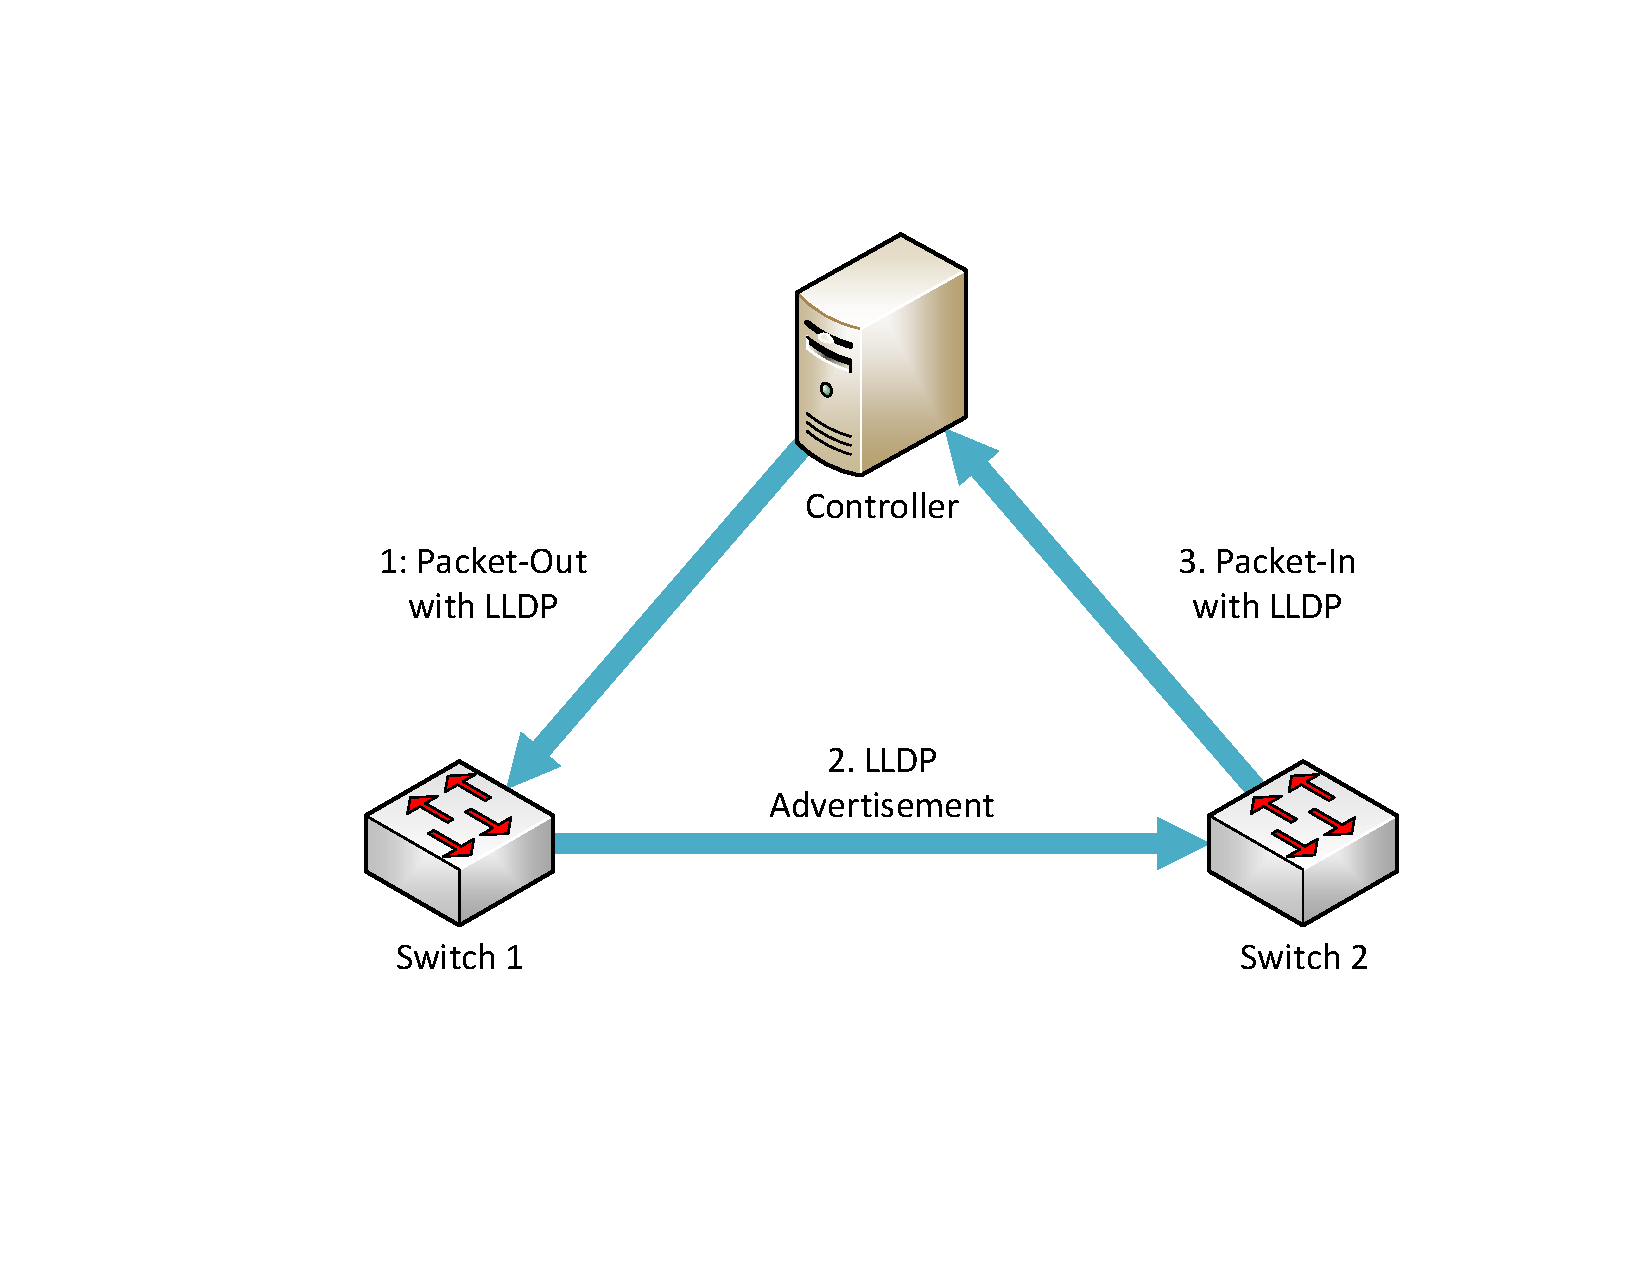
\includegraphics[trim = 50mm 50mm 40mm 35mm, clip, scale = 0.5]{./link.pdf}
				\caption{Link Discovery in OpenFlow Networks}
				\label{link}
			\end{figure}
			
		\item \textbf{Host Discovery:} When a packet from a host reaches to the switch it connected to, the switch matches the packet with existing rules. For the first packet from a host, there would be no matching rule. Hence, the switch sends this packet to controller asking for a rule. By inspecting the packet the controllers learns the location of the host. Since, a host might move from one switch to another or DHCP may reassign IP to hosts, Panorama maintains a timer for each discovered hosts. A clean up is performed periodically. The duration of this period is greater than expected hard timeouts. Information stored for each discovered host includes:
		\begin{enumerate}
			\item IP Address.
			\item MAC Address.
			\item Time, which defines the time when the host was discovered.
		\end{enumerate}
	\end{enumerate}
	
	\section{Port Stats}
	OpenFlow PORT\_STATS messages are used to obtain per port statistics for every port on a switch. When a switch receives such a request, it replies with number of transmitted packets, transmitted bytes, transmit error, packet dropped by TX, collisions, received packets, received bytes, receive errors, packet dropped by RX, packets with RX overrun, frame alignment errors, CRC errors for each of its port.
	\begin{table}[!htbp]
		\centering
		\label{port}
		\begin{tabular}{|c|c|c|c|c|c|c|c|c|c|c|c|c|}
			\hline
\rotatebox{90}{port\_no} & \rotatebox{90}{tx\_packets} & \rotatebox{90}{tx\_bytes} & \rotatebox{90}{tx\_errors} & \rotatebox{90}{tx\_dropped} & \rotatebox{90}{collisions} & \rotatebox{90}{rx\_packets} & \rotatebox{90}{rx\_bytes} & \rotatebox{90}{rx\_errors} & \rotatebox{90}{rx\_dropped} & \rotatebox{90}{rx\_over\_err} & \rotatebox{90}{rx\_frame\_err} & \rotatebox{90}{rx\_crc\_err} \\ \hline
		\end{tabular}
		\caption{Main components of Port Statistics}
	\end{table}

	\section{Aggregate Stats}
	Aggregate Statistics for a switch include total number of flows installed, total number of packets and total number of bytes processed by the switch.
	\begin{table}[!htbp]
		\centering
		\label{aggr}
		\begin{tabular}{|c|c|c|}
			\hline
			 flow\_count & packet\_count & byte\_count  \\ \hline
		\end{tabular}
		\caption{Main components of Aggregate Statistics}
	\end{table}
	
	\section{Flow Stats}
	OpenFlow FLOW\_STATS messages are used to obtain per flow statistics for every flow rule installed on a switch. A flow table consists of several flow entries, and each flow table entry contains:
	\begin{table}[!htbp]
		\centering
		\label{flow_entry}
		\begin{tabular}{|c|c|c|c|c|c|}
			\hline
			Match Fields & Priority & Counters & Instructions & Timeouts & Cookie \\ \hline
		\end{tabular}
		\caption{Main components of a flow entry}
	\end{table}
	\begin{enumerate}
		\item \textbf{Match Fields:} These are the field against which packets are matched. A match field may be exact or may be wild-carded (match any value).
		\begin{table}[!htbp]
			\centering
			\label{match}
			\begin{tabular}{|c|c|c|c|c|c|c|c|c|c|c|c|c|c|}
				\hline
				\rotatebox{90}{Ingress Port} & \rotatebox{90}{Ether Src.} & \rotatebox{90}{Ether Dst.} & \rotatebox{90}{Ether Type} & \rotatebox{90}{VLAN Id} & \rotatebox{90}{VLAN Priority} & \rotatebox{90}{MPLS Label} & \rotatebox{90}{MPLS Traffic Class } & \rotatebox{90}{IP Src.} & \rotatebox{90}{IP Dst.} & \rotatebox{90}{IP Proto.} & \rotatebox{90}{IP ToS} & \rotatebox{90}{Transp. Src. Port} & \rotatebox{90}{Transp. Dst. Port} \\ \hline
			\end{tabular}
			\caption{Main components of the Match field}
		\end{table}
		\item \textbf{Priority:} It is an integer number that defines the matching precedence of the flow entry. The higher the number, the higher the priority.
		\item \textbf{Counters:} Counters are updated when packets are matched. Counters are maintained for each port, queue, flow entry, flow table, meter, meter band and group.
		\item \textbf{Instructions:} An instruction is executed, when a packet matches a flow entry. Instruction may be ``Required Instruction'' or ``Optional Instruction''. Instructions either modify pipeline processing or contain a set of actions to be performed for the match.
		\item \textbf{Timeouts:} A flow entry may have two type of timeouts hard and idle. Depending upon the type of timeouts, they define either the maximum amount of time or idle time before a flow is evicted by a switch.
		\item \textbf{Cookies:} Controller usages cookies to filter flow modification, statistics and deletion but not at the time of processing packets.
	\end{enumerate}
An OpenFlow switch should essentially have at least one flow table, and it can optionally have more than one flow tables as well. The advantage is that many network deployment require orthogonal processing of packets (e.g., QoS, ACL and routing). Using a single to force all those processing creates a huge rule-set. Using multiple tables may properly decouple those processing. Packet processing through multiple flow tables is called the OpenFlow pipeline processing. Panorama reports pipeline processing in the instructions field.
	
	\section{Link Throughput}
	One of the important aspect of network monitoring is to estimate throughput over network links. Panorama calculates uni-directional and bi-directional throughput between a pair links using the PORT\_STATS received from the switches. Calculation of uni-directional and bi-directional throughput in bits per second (bps) is shown in Eq. \ref{eq_uni} and Eq. \ref{eq_bi} respectively. 
		\begin{figure}[!htbp]
			\centering
			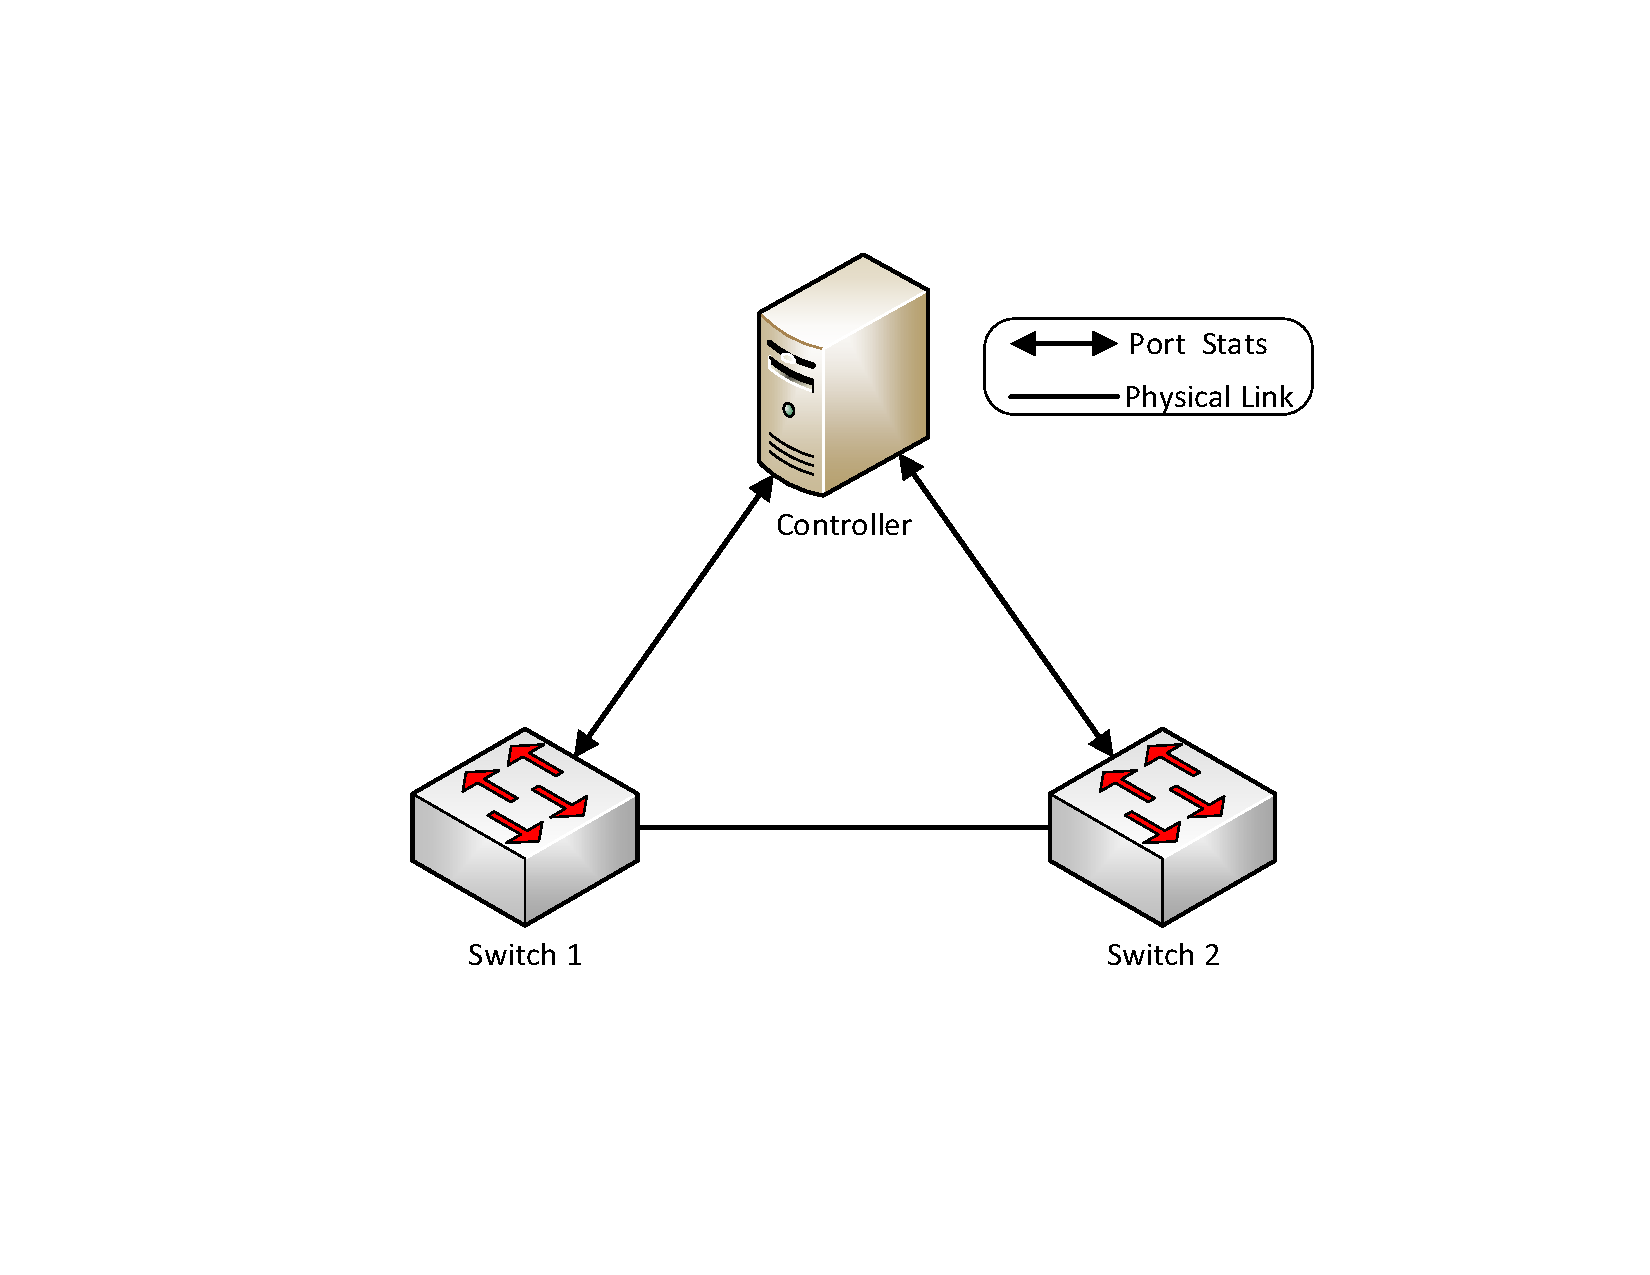
\includegraphics[trim = 40mm 50mm 40mm 40mm, clip, scale=.55]{throughput.pdf}
			\caption[]{Measuring link throughput}
		\end{figure}
		\begin{equation}
		\label{eq_uni}
		Throughput^{Uni}_{S1 \rightarrow S2} = (Cur_{tx\_bytes}^{S1} - Pre_{tx\_bytes}^{S1}) * 8.0 / (Cur_{time}^{S1} - Pre_{time}^{S1})
		\end{equation}
		\begin{equation}
		\label{eq_bi}		
		Throughput^{Bi}_{S1 \leftrightarrow S2} = (Cur^{S1}_{(tx + rx)\_bytes} - Pre^{S1}_{(tx + rx)\_bytes}) * 8.0 / (Cur^{S1}_{time} - Pre^{S1}_{time})
		\end{equation}

	\chapter{Installation}
	\section{Prerequisites}
	Panorama requires following packages to be pre-installed on the system:
	\begin{enumerate}
		\item POX \cite{POX}
		\item OpenFlow 1.0
		\item Python 2.7
		\item Web browser with javascript support.
	\end{enumerate}
	\section{Setting-up the Environment}
	If not already done, set path to \texttt{pox.py} under pox directory (\texttt{$\sim$/pox/}) in your \textit{\$PATH} variable. To set the path through terminal write:
		\texttt{\\~\\
		\$ PATH=\$PATH:$\sim$/pox/\\
		\$ export PATH}
	\section{Getting the Project Files}
	Get the project code from \textcolor{blue}{\href{Source to GIT}{git repository}} and copy the project directory under pox (\texttt{$\sim$/pox/ext/}).
		
	\chapter{How to Start}
	Panorama can be launched either manually or automatically.
	\begin{enumerate}
		\item \textbf{Manual Execution:} 
		\begin{enumerate}
			\item Open a new terminal and run a controller module. This module provides forwarding rules. You may run your own controller module as well.
			\texttt{\\~\\
				\$ cd pox\\
				\$ pox.py forwarding.l2\_learning}\\
			\item Open another terminal and run the monitoring module.
			\texttt{\\~\\
				\$ cd (project working directory i.e.~$\sim$/pox/ext/panorama)\\
				\$ pox.py openflow.of\_01 --port=5566 panorama.panorama}\\
			\item Open another terminal and start a network in Mininet \cite{Mininet, lantz2010network}. You may also create your own custom topology (see Appendix \ref{script}) in which OpenFlow enabled switches connect to both controller module and monitoring module.
			\texttt{\\~\\
				\$ cd (project working directory i.e.~$\sim$/pox/ext/panorama)\\
				\$ sudo python topology/panorama\_mininet.py}\\
			
			\item If a browser window/tab doesn't come up automatically, open a browser window/tab and navigate to localhost.
			\texttt{\\~\\http://localhost:8080/}\\
		\end{enumerate}				
		
		\item \textbf{Automatic Execution:} Simply run the bash script.
			\texttt{\\~\\
			\$ cd (project working directory i.e.~$\sim$/pox/ext/panorama)\\
			\$ bash launch.sh
			}
	\end{enumerate}
	\chapter{Experiment and Verification}
%	Panorama is tested in emulation environment as well as on physical testbed. The emulation was done on a laptop with AMD A4-5000 APU with Radeon (TM) HD Graphics and 4 GB of RAM. Mininet is used as a network emulator. To verify dpctl \cite{dpctl} utility is used. The physical testbed comprises of an HP Aruba 5406R zl2 Switch with Panorama running on a PC with 4th Gen Intel (R) Core i3 processor and 4GB of RAM. Appendix \ref{screenshots} shows the captured screen-shots.
	
	Panorama is tested in emulation environment as well as on physical testbed. The emulation was done using Mininet as the network emulator on a laptop with following specification: 
	\begin{itemize}
		\item[-] AMD A4-5000 1.5 GHz Quad Core APU with Radeon HD Graphics
		\item[-] 4 GB of RAM
		\item[-] 500 GB HDD 
	\end{itemize}

	The physical testbed comprises of an HP Aruba 5406R zl2 Switch with Panorama running on a PC. To verify dpctl \cite{dpctl} utility is used. Appendix \ref{screenshots} shows the captured screen-shots. The specification of the PC are listed below.
	
	\begin{itemize}
		\item[-] 4th Gen Intel Core i3 processor with Intel HD Graphics
		\item[-] 4 GB of RAM
		\item[-] 500 GB HDD
	\end{itemize}
	
	\chapter{Future Work}
		Delay introduced by a link and link loss play a crucial role in Quality-of-Service provisioning. The work in \cite{gourov2013network} demonstrates mechanisms to measure link delay and loss. In future, we shall incorporate those measurements and we also hope to develop Panorama as controller independent module.
		\section{Link Delay}
		The controller injects probe packets to calculate delay on the links. It generates UDP packet and sends it to Switch 1. The controller also installs a new rule in flow table of Switch 1 instructing Switch 1 to send this probe packet to Switch 2. At $t1$ the packet flows from Switch 1 to Switch 2. Since no matching rule is installed in flow table of Switch 2, the switch returns the packet to the controller at $t2$. The controller receives this packet at $t3$. The controller keeps constant connection with every switch, hence, it knows the delay between it and the switches, as shown in Eq. \ref{delay1}. This enables controller to estimate the delay	between every pair of switches, as shown in Eq. \ref{delay2}.
		\begin{equation}
		\label{delay1}
		T1 = T3 = 0.5 * (T_b - T_a)
		\end{equation}
		\vspace{-10mm}
		\begin{align}
		T_a = OF_{request\_send\_time} ~and~ T_b = OF_{reply\_receive\_time} \nonumber
		\end{align}
		\begin{equation}
		\label{delay2}
		Time_{total} = T1 + T2 + T3 \Rightarrow T2 = Time_{total} - T1 - T3
		\end{equation}

		\begin{figure}[!htbp]
			\label{delay}
			\centering
			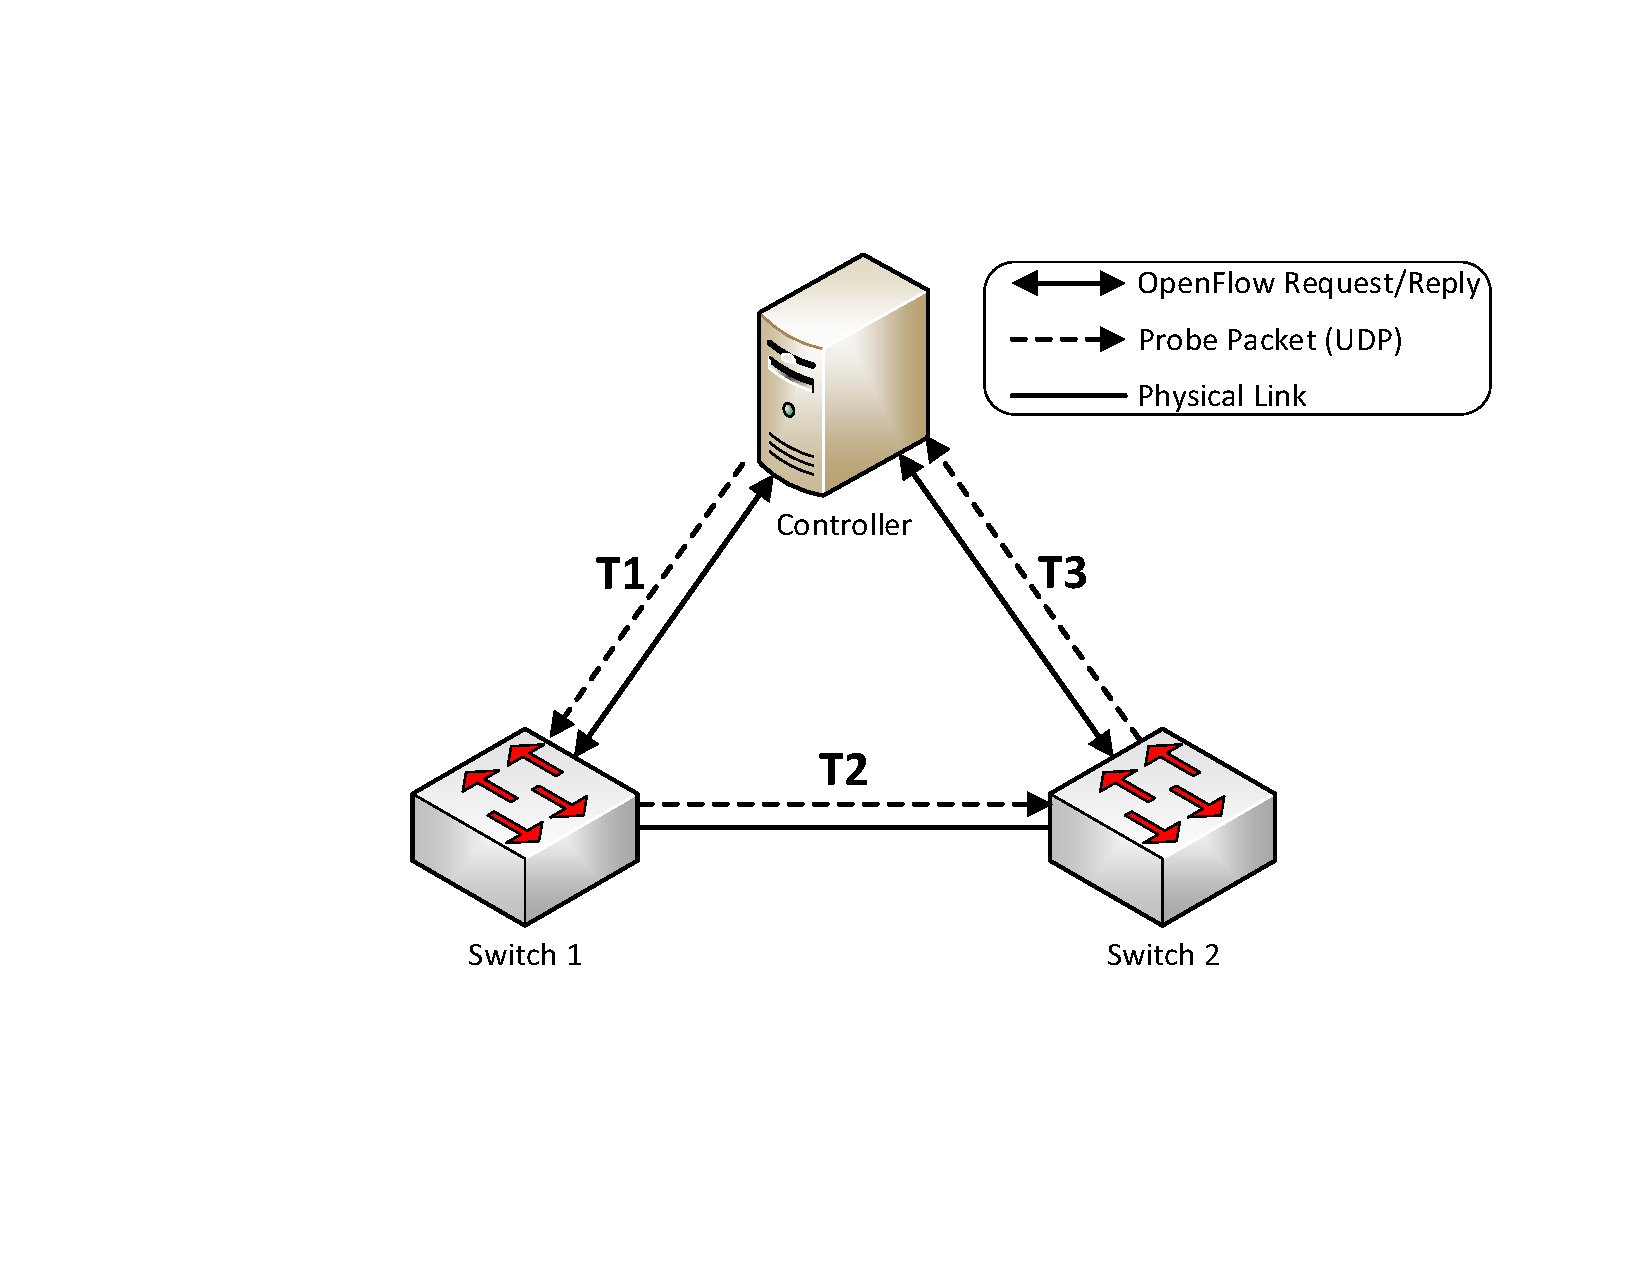
\includegraphics[trim = 40mm 50mm 15mm 40mm, clip, scale=.5]{delay.pdf}
			\caption[]{Measuring link delay}
		\end{figure}		
	
	\section{Link Loss}\ref{loss}
	When a flow arrives and the switch does not have any matching rule installed, the first packet of the flow is sent to the controller. The controller instructs the switch what to do with	the packet. It instructs the switch by installing table rules on the switch for the flow. As soon as the flow expires, the switch indicates this event to the controller. The entire process is illustrated in Figure \ref{loss}. The flow is installed at time $t1$ using FLOW\_MOD messages. At time $t2$ and $t3$, the controller receives FLOW\_REMOVED messages from Switch 1 and Switch 2 respectively. Those messages include specific statistics for the flow, e.g., the number of packets, bytes. The packet-loss can be measured on the basis of those statistics, as shown in Eq. \ref{eq_loss}.
	\begin{equation}
	\label{eq_loss}
	Loss_\% = (1-packets_{Switch2}/packets_{Switch1})*100
	\end{equation}
	\begin{figure}[!htbp]
		\centering
		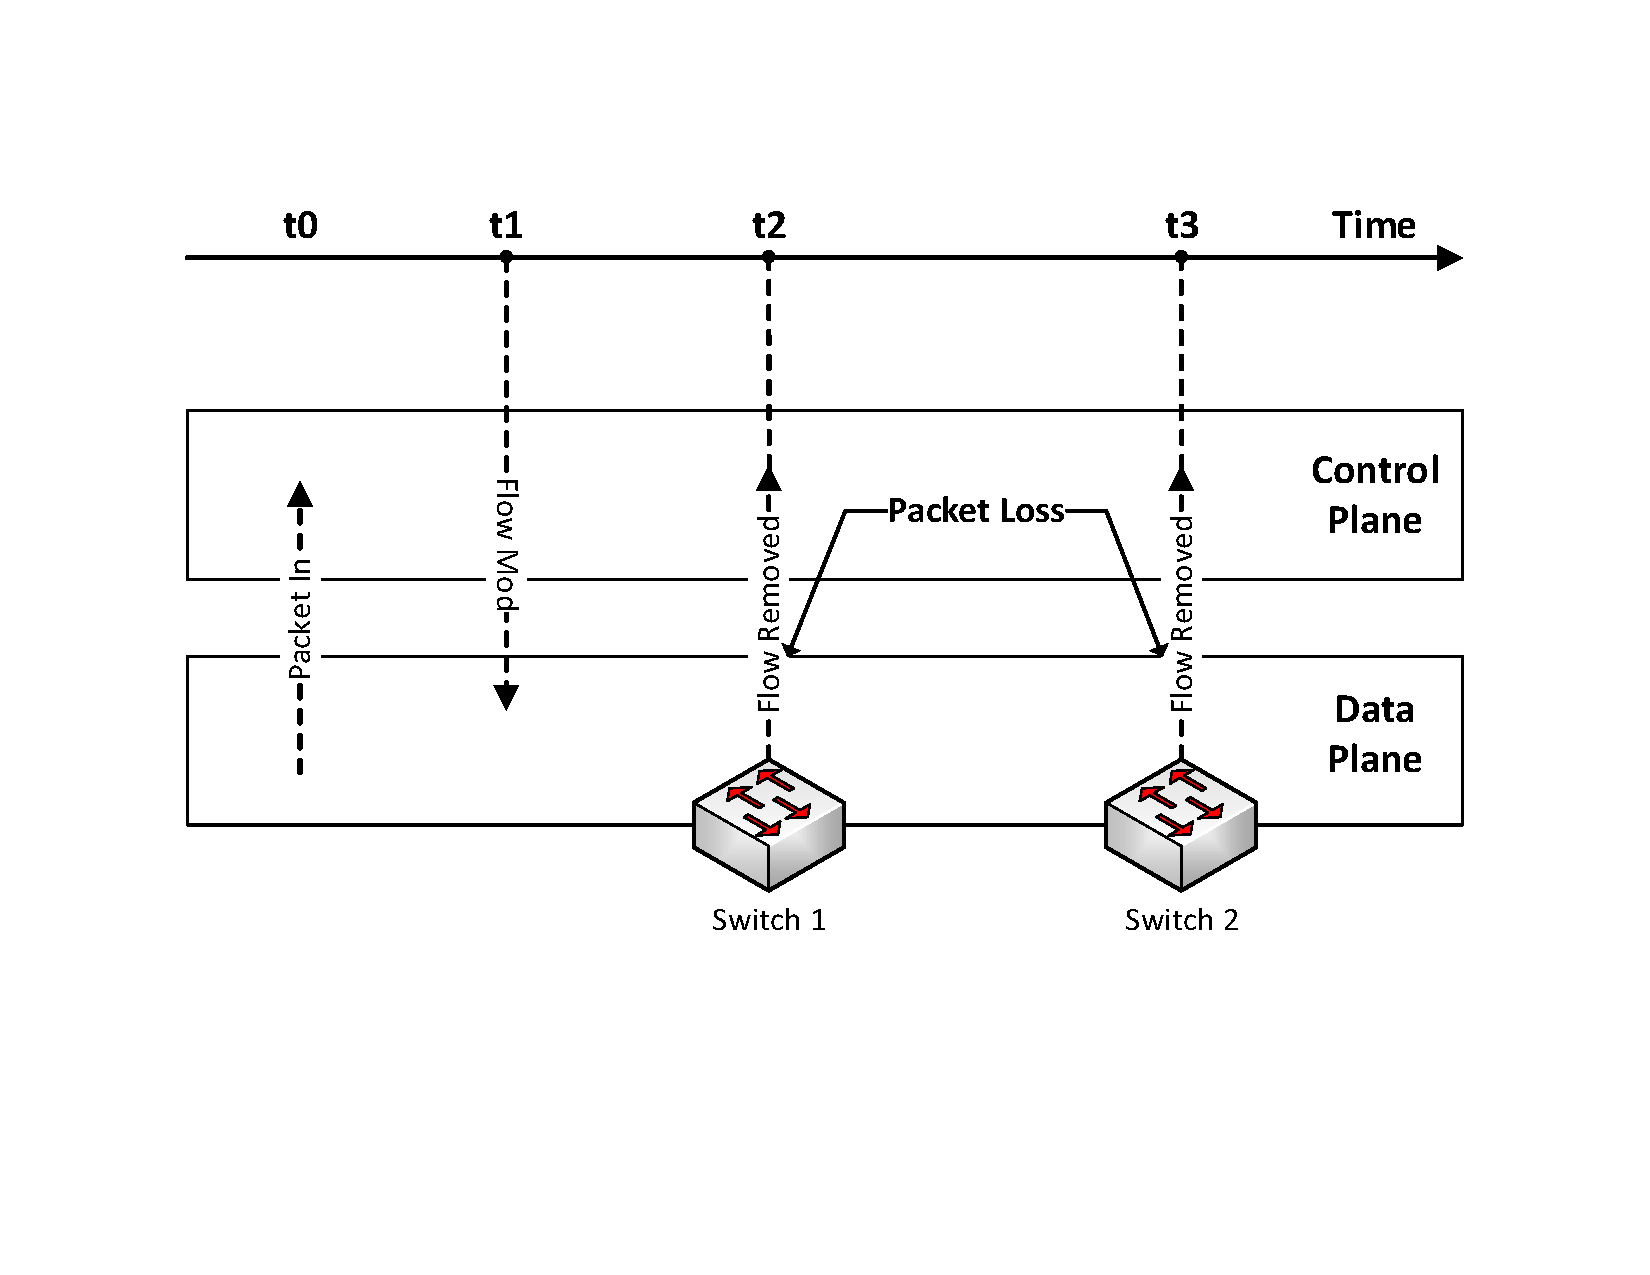
\includegraphics[trim = 30mm 55mm 25mm 35mm, clip, scale=.65]{loss.pdf}
		\caption[]{Measuring link loss}
		\label{loss}
	\end{figure}
	

\pagebreak
\addcontentsline{toc}{chapter}{Bibliography}
\bibliographystyle{IEEEtran}
\bibliography{bib}
\begin{appendices}
	\chapter{Custom Topology Script}
	\label{script}
	\lstinputlisting[language = Python,basicstyle=\footnotesize, showstringspaces=false,tabsize=1,breaklines=true,breakatwhitespace=false,frame=single,captionpos=b,caption=Sample topology script]{./scripts/panorama_mininet.py}
	\chapter{Screenshots}
		\label{screenshots}
			\begin{figure}[!htbp]
				\centering
				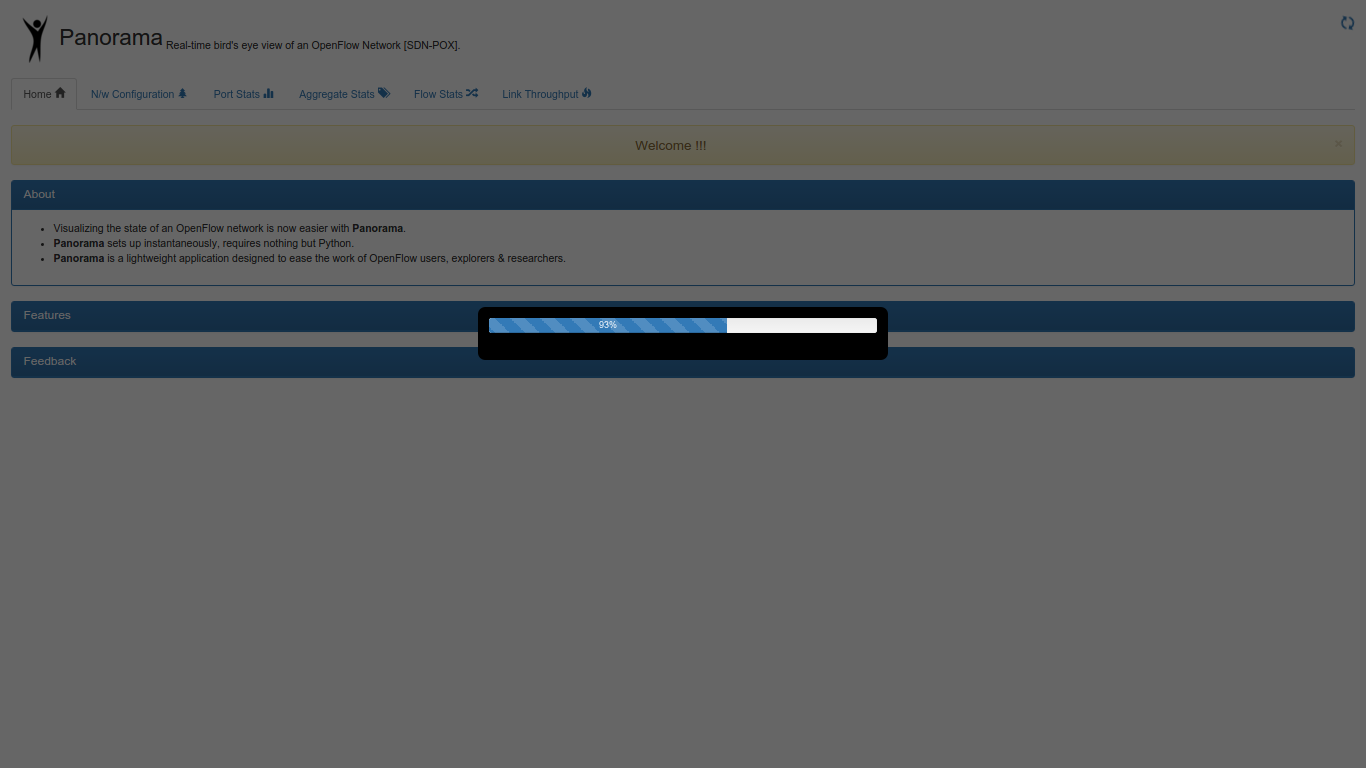
\includegraphics[trim = 03mm 70mm 03mm 0mm, clip, scale=.3]{loading}
				\caption[]{Loading}
			\end{figure}
		\begin{figure}[!htbp]
			\centering
			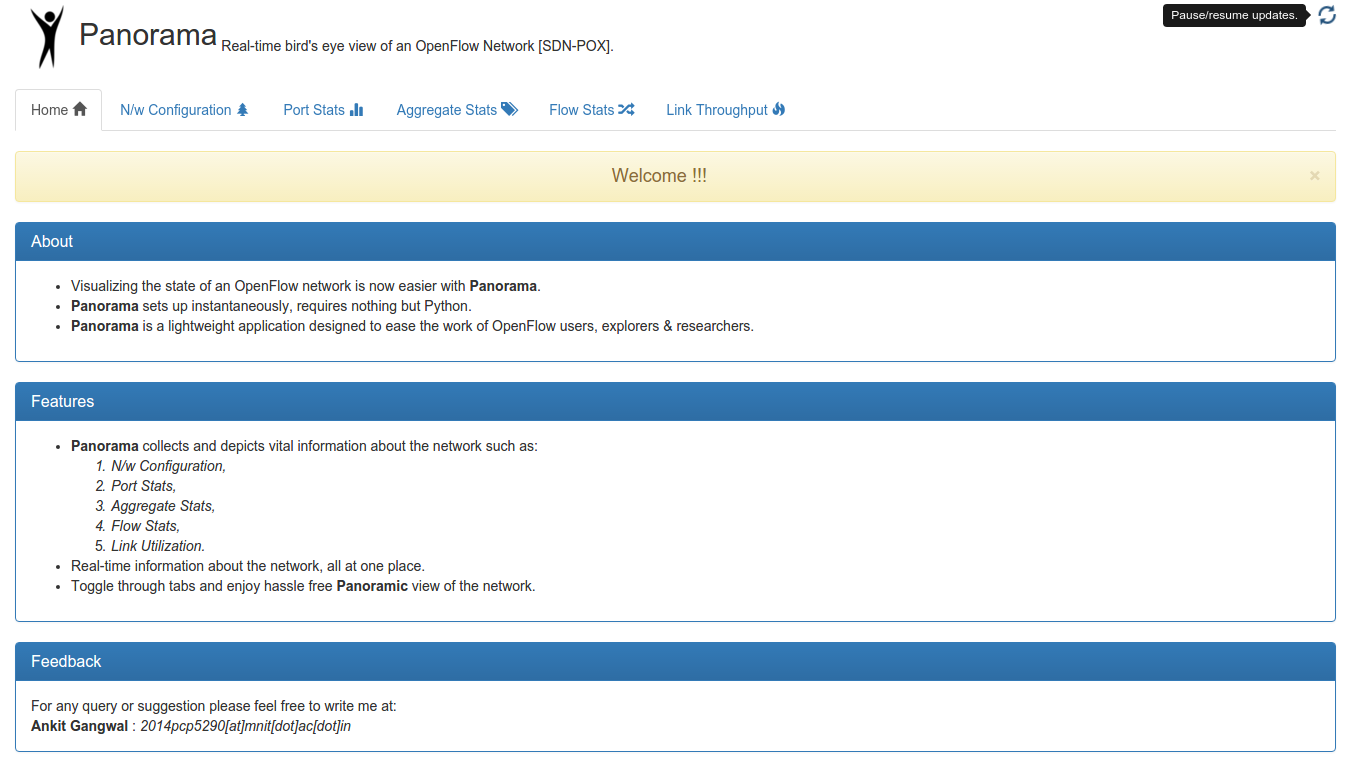
\includegraphics[trim = 5mm 0mm 0mm 0mm, clip, scale=.3]{home}
			\caption[]{Home tab}
		\end{figure}
		
		\begin{sidewaysfigure}[!htbp]
			\centering
			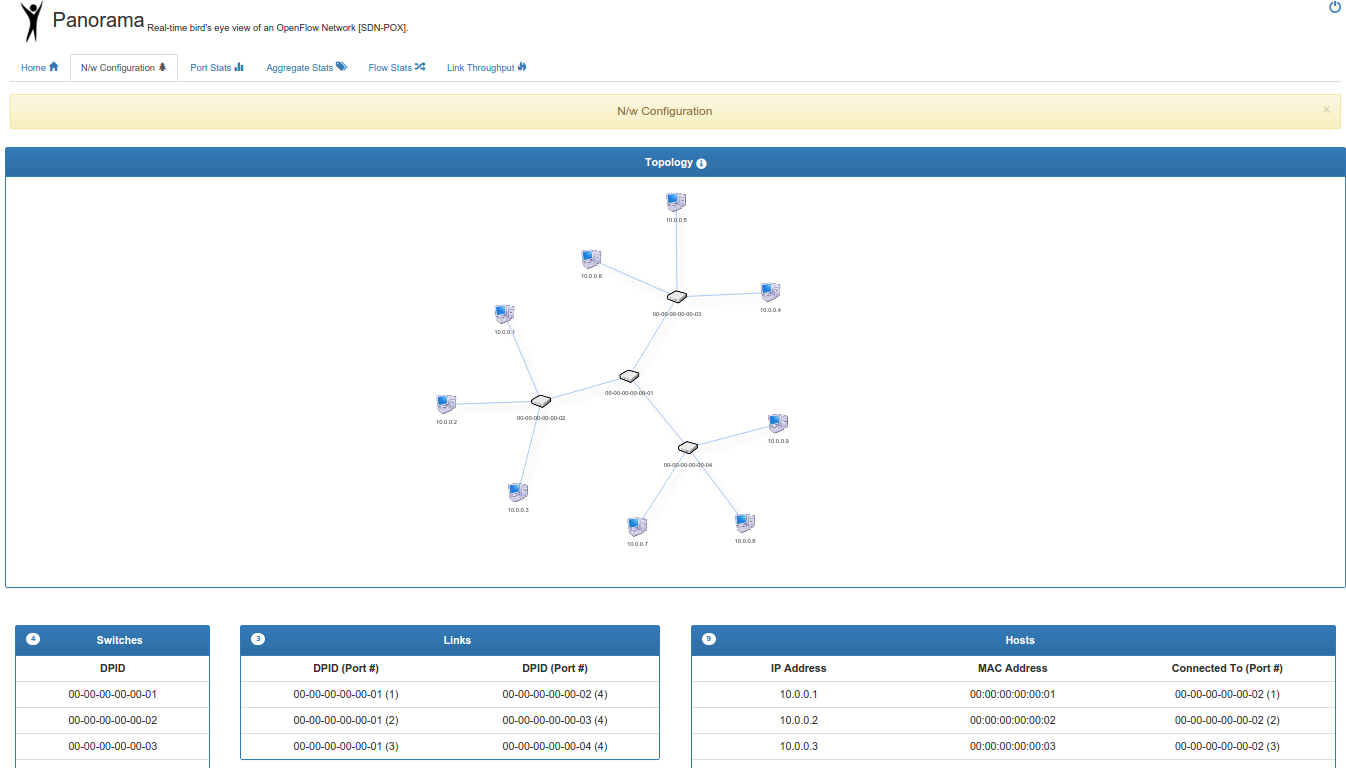
\includegraphics[trim = 0mm 0mm 0mm 0mm, clip, width=\columnwidth]{topo}
			\caption[]{N/w Configuration tab}
		\end{sidewaysfigure}

		\begin{sidewaysfigure}[!htbp]
			\centering
			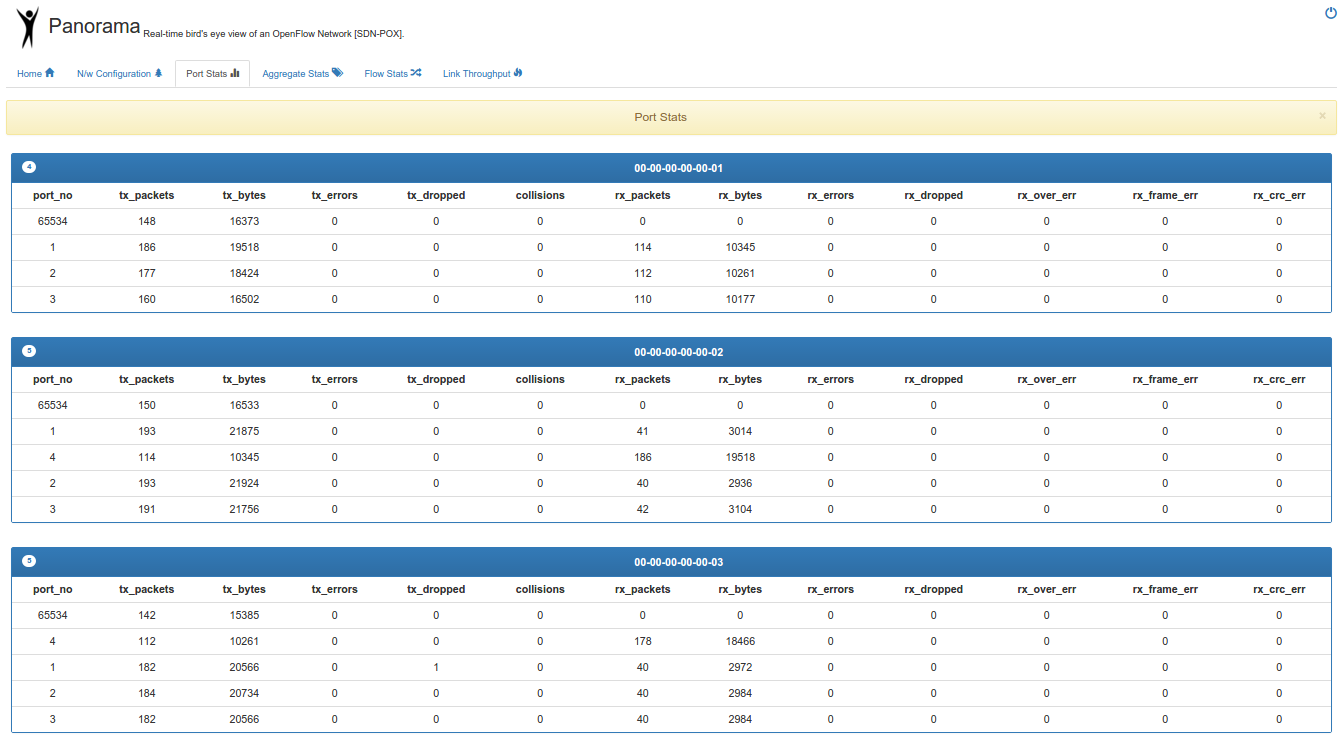
\includegraphics[trim = 0mm 0mm 0mm 0mm, clip, width=\columnwidth]{port}
			\caption[]{Port Stats tab}
		\end{sidewaysfigure}

		\begin{sidewaysfigure}[!htbp]
			\centering
			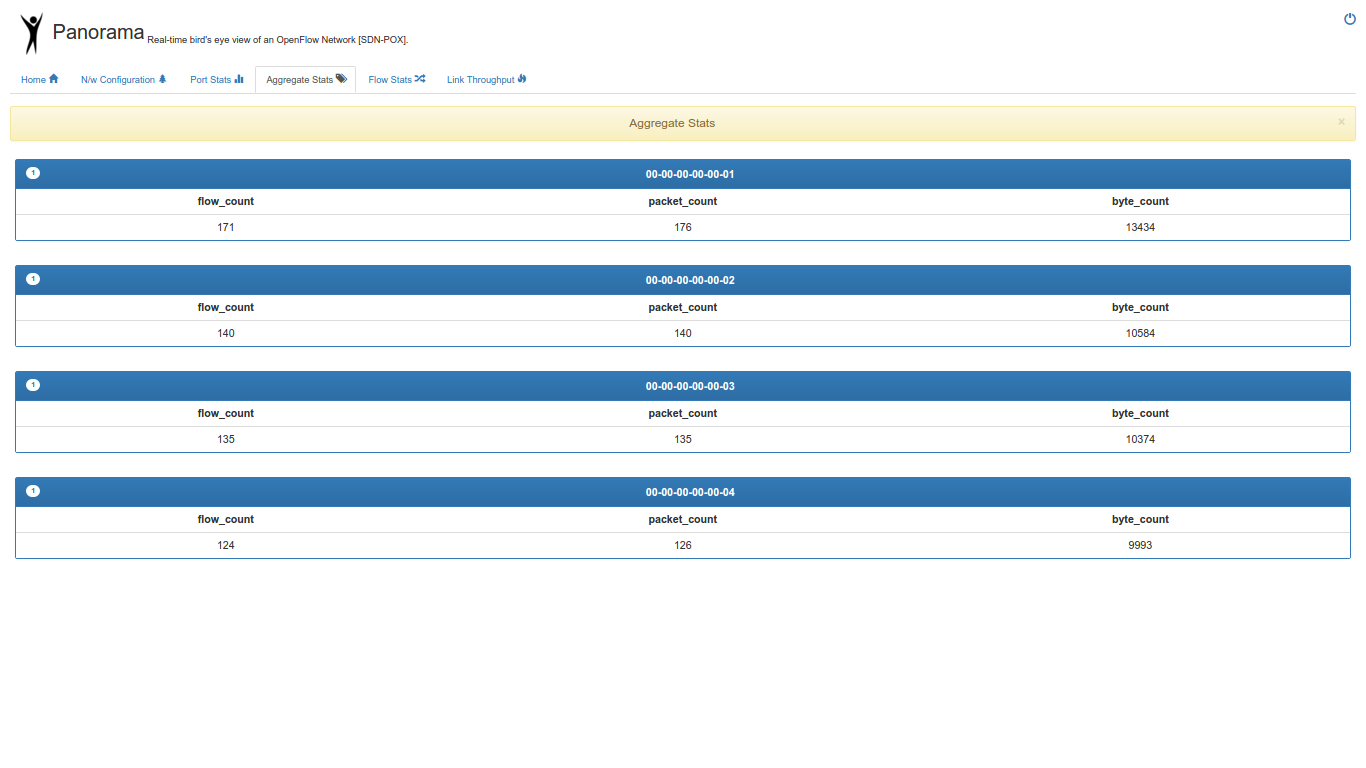
\includegraphics[trim = 0mm 60mm 0mm 0mm, clip, width=\columnwidth]{agg}
			\caption[]{Aggregate Stats tab}
		\end{sidewaysfigure}
		
		\begin{sidewaysfigure}[!htbp]
			\centering
			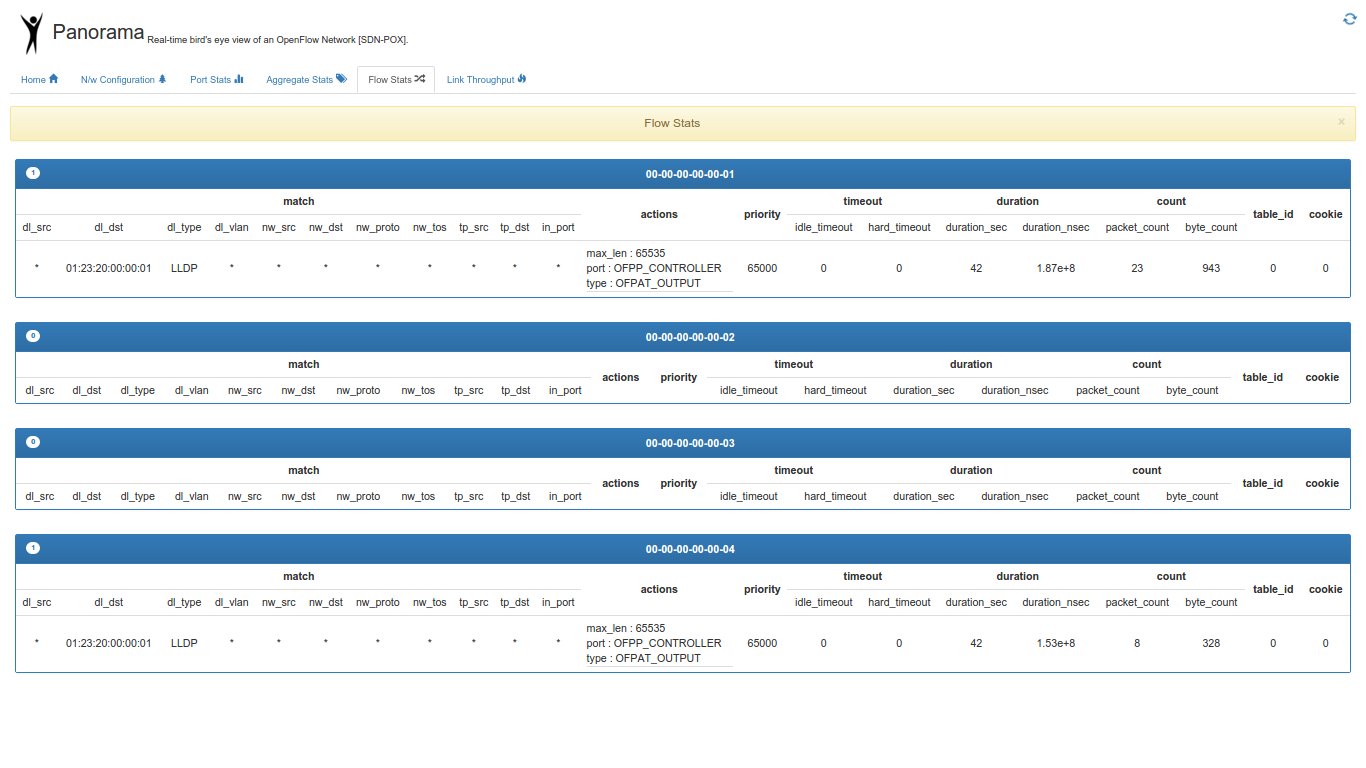
\includegraphics[trim = 0mm 0mm 0mm 0mm, clip, width=\columnwidth]{flow}
			\caption[]{Flow Stats tab}
		\end{sidewaysfigure}

		\begin{sidewaysfigure}[!htbp]
			\centering
			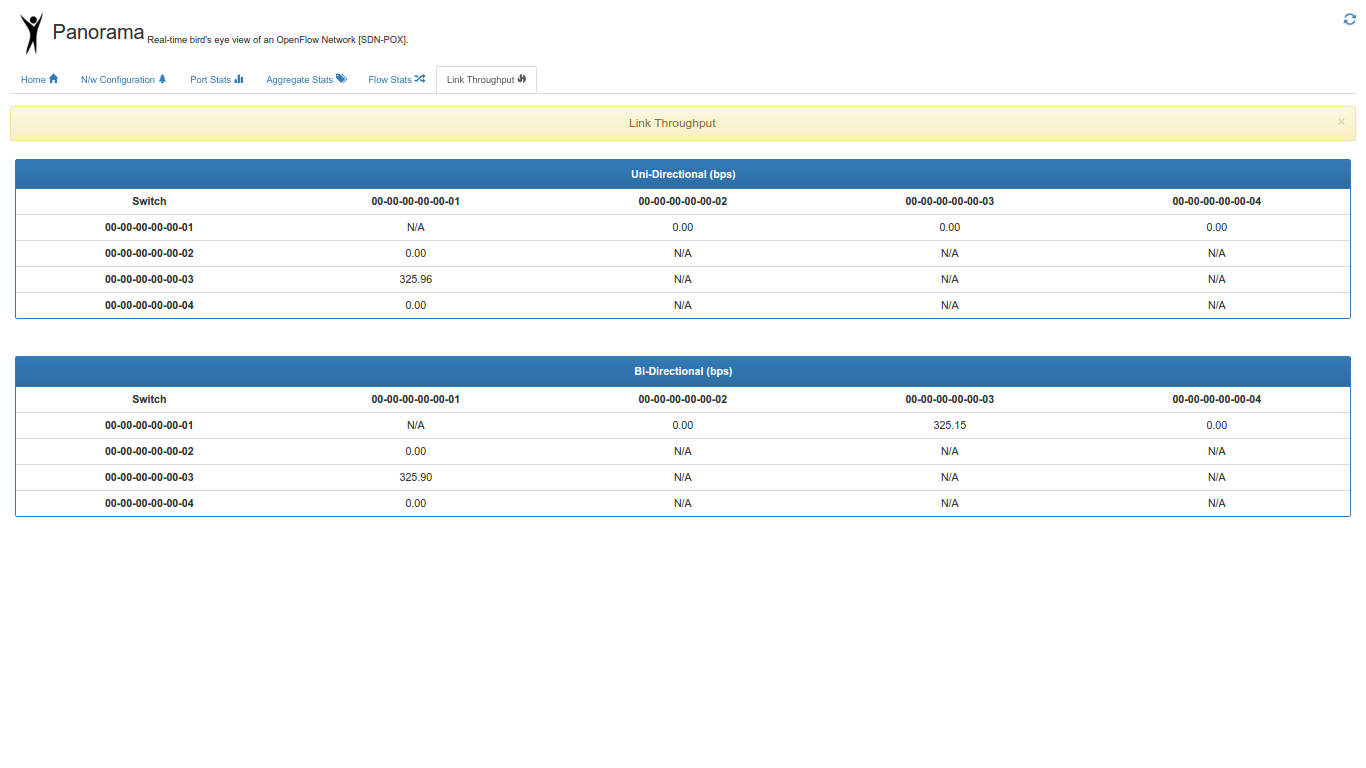
\includegraphics[trim = 0mm 60mm 0mm 0mm, clip, width=\columnwidth]{uti}
			\caption[]{Link Throughput tab}
		\end{sidewaysfigure}
\end{appendices}


\end{document}